\documentclass[aps,prd,twocolumn,nofootinbib]{revtex4-1}
\usepackage{amsmath}
\usepackage{graphicx}
\usepackage{subfig}
\usepackage{epsfig}
\usepackage{listings}
\usepackage[hidelinks,hyperfootnotes=false,bookmarks=false]{hyperref}
\usepackage[colorinlistoftodos]{todonotes}
\usepackage{verbatim}
\usepackage{float}
\begin{document}
\title{A Survey of Sterile Neutrinos}
\author{Douglas Davis}
\author{Matthew Epland}
\author{Justin Raybern}
\author{Pingchuan Zhao}
\affiliation{Department of Physics, Duke University, Durham, NC 27707, USA}
\date{\today}
\begin{abstract}
  xxxxxxxxxxxxxxxxxxxxxxxxxxxxxxxxx xxxxxxxxxxxxxxxxxxxxxxxxxxxxxxxxxxxxxxxxxx xxxxxxxxxxxxxxxxxxxxxxxxxxxxxxxxxxxxxxxxxxxxxxxxxxxxxxxxxxxxxxxxxxxxxxxxxxx xxxxxxxxxxxxxxxxxxxxxxxxxxxxxxxxxxxxxxxxxx xxxxxxxxxxxxxxxxxxxxxxxxxxxxxxxxxxxx xxxxxxxxxxxxxxxxxxxxxxxxxxxxxxxxxxxxxxxxxx xxxxxxxxxxxxxxxxxxxxxxxxxxxxxxxxxxxxxxxxxx xxxxxxxxxxxxxxxxxxxxxxxxxxxxxxxxxxxxx xxxxxxxxxxxxxxxxxxxxxxxxxxxxxxxxxxxxxxxxxx xxxxxxxxxxxxxxxxxxxxxxxxxxxxxxxxxxxxxxxxxx xxxxxxxxxxxxxxxxxxxxx
\end{abstract}\maketitle
\section{Theory}
\label{sec:theory}
xxxxxxxx xxxxxx xxxxxxxx xxxxxx xxxxxxxx xxxxxx xxxxxxxx xxxxxx xxxxxxxx xxxxxx xxxxxxxx xxxxxx xxxxxxxx xxxxxx
\subsection{Theory Ping}
xxxxxxxx xxxxxx xxxxxxxx xxxxxx xxxxxxxx xxxxxx xxxxxxxx xxxxxx xxxxxxxx xxxxxx xxxxxxxx xxxxxx xxxxxxxx xxxxxx
\subsection{Theory Justin}
xxxxxxxx xxxxxx xxxxxxxx xxxxxx xxxxxxxx xxxxxx xxxxxxxx xxxxxx xxxxxxxx xxxxxx xxxxxxxx xxxxxx xxxxxxxx xxxxxx
\section{Previous Experimental Efforts}
There exists considerable experimental evidence for the existence of a fourth neutrino at energy scales in the eV range. The sources for evidence include the short baseline neutrino oscillation experiments LSND (Liquid Scintillator Neutrino Detector) at Los Alamos~\cite{LSND}, and MiniBooNE (Mini Booster Neutrino Experiment) at Fermilab~\cite{mini1,mini2}. There is also the reactor neutrino anomaly~\cite{reactor_anom1}, and also in the radioactive source calibrations for the solar neutrino experiments GALLEX~\cite{gallex1,gallex2} and SAGE~\cite{sage1,sage2}.
\subsection{LSND}
The LSND experiment was developed to search for $\overline{\nu}_\mu \rightarrow \overline{\nu}_e$ oscillations. The source of $\overline{\nu}_\mu$ was the decay at rest (DAR) of $\mu^+$. LSND used a proton beam on a target to produce pions. The decay chain was as follows:
\begin{align}
  \begin{split}
    \pi^+ &\rightarrow \mu^+  \nu_\mu, \\
    \mu^+ &\rightarrow e^+  \nu_e  \overline{\nu}_\mu.
  \end{split}
\end{align}
The $\overline{\nu}_e$ events were detected through the interaction:
\begin{align}
  \overline{\nu}_e  p \rightarrow e^+ n,
\end{align}
inside of a large Cherenkov detector filled with liquid scintillator, utilizing 1280 phototubes. Figure~\ref{fig:lsnd_miniboone}(L) shows the excess of $\overline{\nu}_e$ events observed by LSND. The observation was $87.9\pm 22.4\pm6$ events over expected background. Their final result claimed the existence of $\overline{\nu}_\mu\rightarrow\overline{\nu}_e$ oscillations at $\Delta m^2 \sim 1\text{ eV}$ with 3.8$\sigma$. This is in heavy conflict with the existing three light flavor neutrino model supported by atmospheric and solar neutrino oscillation experiments, as well as measurements at LEP predicting $N=2.984\pm0.0082$ for weakly interacting neutrino flavors. Therefore, at least one ``sterile'' neutrino is required.
\begin{figure*}
  \centering
  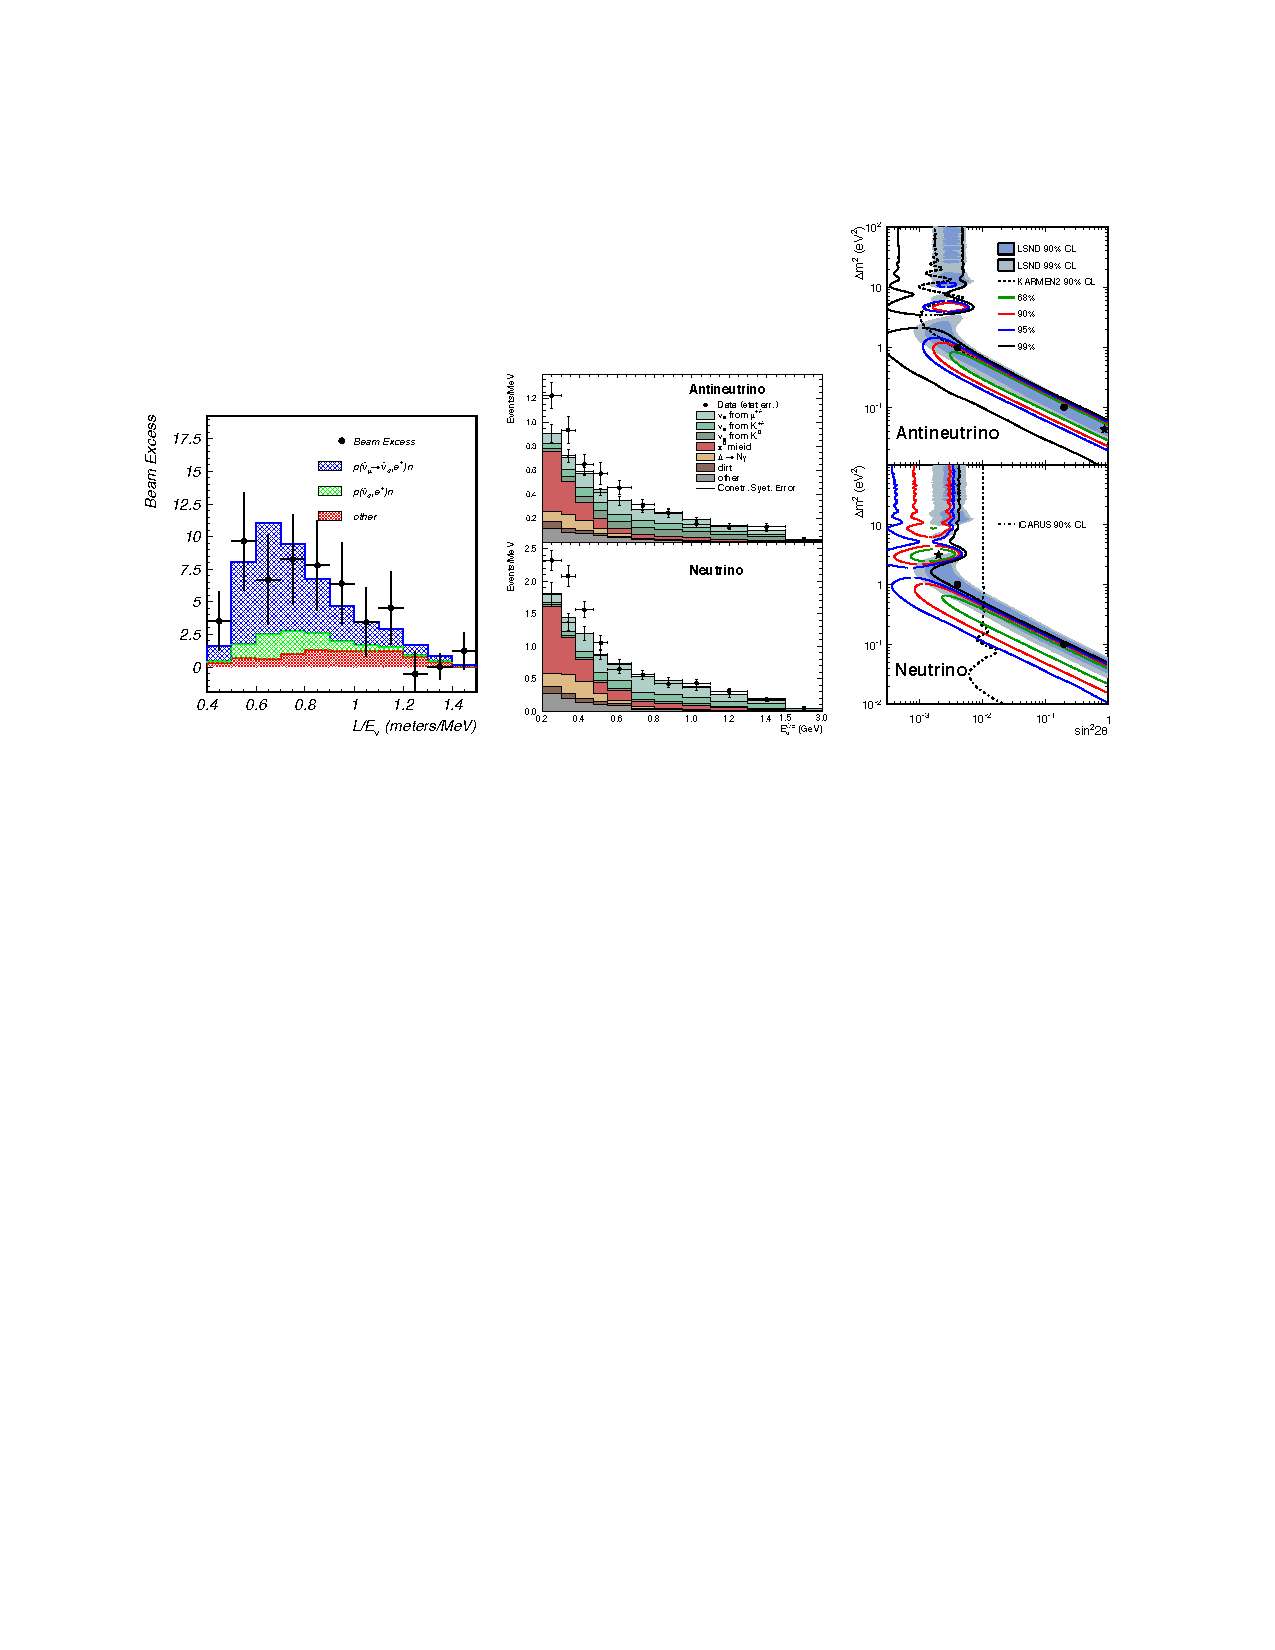
\includegraphics[width=1\textwidth]{../figures/lsnd_miniboone.pdf}
  \caption{(L) From the LSND Experiment~\cite{LSND}. The expected number of events is represented by the red and green histograms, the blue histogram agrees with the data and models $\overline{\nu}_{\mu}\rightarrow \overline{\nu}_e$ oscillation. (C) The MiniBooNE electron event excess in neutrino and anti-neutrino sector~\cite{mini2}. (R) The MiniBooNE allowed regions in neutrino and anti neutrino mode, for a 2 neutrino model. Black stars represent the MiniBooNE best fit points for $\Delta m^2$ and $\sin^22\theta$.~\cite{mini2}}
  \label{fig:lsnd_miniboone}
\end{figure*}
\subsection{MiniBooNE}
The MiniBooNE experiment was developed to answer the LSND anomaly. The MiniBooNE detector also used Cherenkov radiation with photomultiplier tubes as their tool for detecting neutrino interactions. The Booster neutrino beam at Fermilab was used to create a $\nu_\mu$ or $\overline{\nu}_\mu$ beam. Protons were accelerated to 8 GeV by the Booster accelerator and were then steered to a beryillium target where a magnetic focusing horn steered pions from the proton on target collisions down the beam line towards the detector; the pions would decay into muons and muon neutrinos between the horn and the detector. Changing the magnetic focusing horn mode allowed for a beam of mostly $\nu_\mu$ or mostly $\overline{\nu}_\mu$ (neutrino or anti neutrino modes). In neutrino mode $\pi^+$ were steered towards the detector, while $\pi^-$ were steered away; and the reverse for anti neutrino mode. This is to utilize the decays:
\begin{align}
  \begin{split}
    \pi^+ &\rightarrow \mu^+\nu_\mu \\
    \pi^- &\rightarrow \mu^-\overline{\nu}_\mu  
  \end{split}
\end{align}
The full dataset from MiniBooNE was consistent with the LSND $\overline{\nu}_e$ excess, and therefore the sterile neutrino hypothesis survives with a best fit $\Delta m^2 \sim 1$ eV.
\subsection{Reactor Anomaly}
reactors are cool.

\section{Current and Future Experimental Efforts}
Due to the number of anomalous results to date sterile neutrino searches have become popular research topics at the majority of contemporary neutrino experiments, both those currently running and those in the design and construction phases.
\subsection{Current}
% Matt
\subsubsection{MINOS/MINOS+}
The MINOS (Main Injector Neutrino Oscillation Search) experiment ran from 2005 to 2012 and its upgraded second run, MINOS+, has taking data since September 2013. The MINOS experiment is a long baseline style detector with a neutrino beam source and near detector at Fermilab and a far detector located in northern Minnesota. Though it's primary physics goals lie in the area of neutrino oscillation measurements, MINOS and MINOS+ are now also running sterile neutrino analysis with their data. MINOS detects sterile nutrinos via their disappearence in neutral-current (NC) and 

The latest results \cite{MINOS+} are still in preprint but 

\subsubsection{T2K}

\subsubsection{Daya Bay}


\subsection{Future}
% Matt
NOVA
MicroBooNE
DUNE (Formerly LBNE)


\section{Conclusions}
xxxxxxxx xxxxxx xxxxxxxx xxxxxx xxxxxxxx xxxxxx xxxxxxxx xxxxxx xxxxxxxx xxxxxx xxxxxxxx xxxxxx xxxxxxxx xxxxxx
who cares

\begin{thebibliography}{9}
\bibitem{LSND}
  A.~Aguilar-Arevalo \emph{et al.} Evidence for neutrino oscillations from the observation of anti-neutrino(electron) appearance in a anti-neutrino(muon) beam. \emph{Phys. Rev. D.}, {\bf 64} 112007, 2001.
\bibitem{mini1}
  A.~Aguilar-Arevalo \emph{et al.} Event Excess in the MiniBooNE Search for $\nu_\mu \rightarrow \nu_e$ Oscillations. \emph{Phys. Rev. Lett.}, {\bf 105} 181801, 2010.
\bibitem{mini2}
  A.~Aguilar-Arevalo \emph{et al.} Improved Search $\nu_\mu \rightarrow \nu_e$ Oscillations in the MiniBooNE Experiment. \emph{Phys. Rev. Lett.}, {\bf 110} 161801, 2013.
\bibitem{reactor_anom1}
  G. Mention, M. Fechner, Th. Lasserre, Th.A. Mueller, D. Lhuillier, \emph{et al.} The Reactor Antineutrino Anomaly. \emph{Phys. Rev. D.}, {\bf 83} 073006, 2011.
\bibitem{reactor_anom2}
  Th. A. Mueller, D. Lhuillier, M. Fallot, A. Letourneau, S. Cormon, \emph{et al.} Improved Predictions of Reactor Antineutrino Spectra. \emph{Phys. Rev. C.}, {\bf 83} 054615, 2011.
\bibitem{gallex1}
  P.~Anselmann~\emph{et al.} First results from the Cr-51 neutrino source experiment with the GALLEX detector. \emph{Phys. Lett. B.}, {\bf 342} 440-450, 1995
\bibitem{gallex2}
  W.~Hampel~\emph{et al.} Final results of the Cr-51 neutrino source experiments in GALLEX. \emph{Phys. Lett. B.}, {\bf 420} 114-126, 1998.
\bibitem{sage1}
  Dzh.~N.~Abdurashitov, V.N.~Gavrin, S.V. Girin, V.V. Gorbachev, Tatiana V. Ibragimova, \emph{et al.} The Russian-American gallium experiment (SAGE) Cr neutrino source measurement. \emph{Phys. Rev. Lett.}, {\bf 77} 4708-4711, 1996.
\bibitem{sage2}
  J.~N.~Abdurashitov~\emph{et al.} Measurement of the response of the Russian-American gallium experiment to neutrinos from a Cr-51 source. \emph{Phys. Rev. C.}, {\bf 59} 2246-2263, 1999.

\bibitem{MINOS+}
  Alexandre B. Sousa~\emph{(for the MINOS and MINOS+ Collaborations)} First MINOS+ Data and New Results from MINOS. arXiv:1502.07715v1 [hep-ex] \url{http://arxiv.org/abs/1502.07715}


\end{thebibliography}

\end{document} %%% end of doc %%%
